\documentclass[a4paper,twoside,10pt,landscape]{article}
\usepackage{multicol}
\usepackage{calc}
\usepackage{ifthen}
\usepackage[landscape]{geometry}
\usepackage{hyperref}
\usepackage{graphicx} % standard LaTeX graphics tool when including figure files
\graphicspath{{images/}}
\usepackage{caption}

% To make this come out properly in landscape mode, do one of the following
% 1.
%  pdflatex latexsheet.tex
%
% 2.
%  latex latexsheet.tex
%  dvips -P pdf  -t landscape latexsheet.dvi
%  ps2pdf latexsheet.ps


% If you're reading this, be prepared for confusion.  Making this was
% a learning experience for me, and it shows.  Much of the placement
% was hacked in; if you make it better, let me know...


% 2008-04
% Changed page margin code to use the geometry package. Also added code for
% conditional page margins, depending on paper size. Thanks to Uwe Ziegenhagen
% for the suggestions.

% 2006-08
% Made changes based on suggestions from Gene Cooperman. <gene at ccs.neu.edu>


% To Do:
% \listoffigures \listoftables
% \setcounter{secnumdepth}{0}


% This sets page margins to .5 inch if using letter paper, and to 1cm
% if using A4 paper. (This probably isn't strictly necessary.)
% If using another size paper, use default 1cm margins.
\ifthenelse{\lengthtest { \paperwidth = 11in}}
	{ \geometry{top=.5in,left=.5in,right=.5in,bottom=.5in} }
	{\ifthenelse{ \lengthtest{ \paperwidth = 297mm}}
		{\geometry{top=1cm,left=1cm,right=1cm,bottom=1cm} }
		{\geometry{top=1cm,left=1cm,right=1cm,bottom=1cm} }
	}

% Turn off header and footer
\pagestyle{empty}
 

% Redefine section commands to use less space
\makeatletter
\renewcommand{\section}{\@startsection{section}{1}{0mm}%
                                {-1ex plus -.5ex minus -.2ex}%
                                {0.5ex plus .2ex}%x
                                {\normalfont\large\bfseries}}
\renewcommand{\subsection}{\@startsection{subsection}{2}{0mm}%
                                {-1explus -.5ex minus -.2ex}%
                                {0.5ex plus .2ex}%
                                {\normalfont\normalsize\bfseries}}
\renewcommand{\subsubsection}{\@startsection{subsubsection}{3}{0mm}%
                                {-1ex plus -.5ex minus -.2ex}%
                                {1ex plus .2ex}%
                                {\normalfont\small\bfseries}}
\makeatother

% Define BibTeX command
\def\BibTeX{{\rm B\kern-.05em{\sc i\kern-.025em b}\kern-.08em
    T\kern-.1667em\lower.7ex\hbox{E}\kern-.125emX}}

% Don't print section numbers
%\setcounter{secnumdepth}{0}


\setlength{\parindent}{0pt}
\setlength{\parskip}{0pt plus 0.5ex}


% -----------------------------------------------------------------------

\begin{document}

\raggedright
\footnotesize
\begin{multicols}{3}


% multicol parameters
% These lengths are set only within the two main columns
%\setlength{\columnseprule}{0.25pt}
\setlength{\premulticols}{1pt}
\setlength{\postmulticols}{1pt}
\setlength{\multicolsep}{1pt}
\setlength{\columnsep}{2pt}

\begin{center}
     \Large{\textbf{Scala Cheat Sheet}} \\
\end{center}


\section{Scala Class Hierarchy}
\begin{center}
    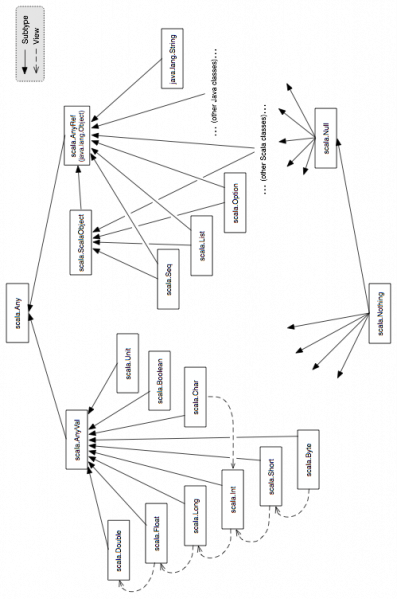
\includegraphics[scale=.80]{classhierarchy.png}
    \captionof{figure}{Scala class hierarchy, source: \url{http://docs.scala-lang.org/tutorials/tour/unified-types.html}}
    \label{fig:scala-class-hierarchy}
\end{center}


\section{Scala Collections Hierarchy}

\begin{center}
    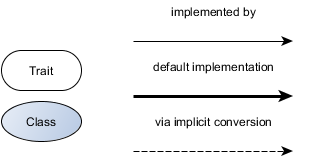
\includegraphics[scale=.50]{legend.png}
\end{center}

\begin{center}
    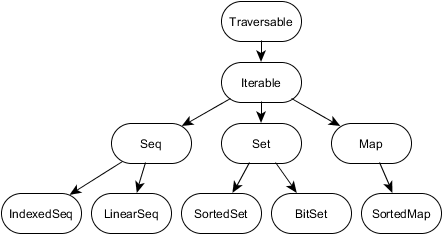
\includegraphics[scale=.50]{scala-collection.png}
    \captionof{figure}{scala.collection}
    \label{fig:scala-collection}
\end{center}

\begin{center}
    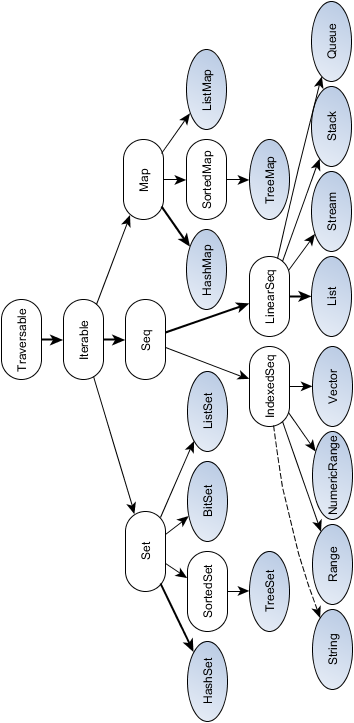
\includegraphics[scale=.65]{scala-collection-immutable.png}
    \captionof{figure}{scala.collection.immutable}
    \label{fig:scala-collection-immutable}
\end{center}

\begin{center}
    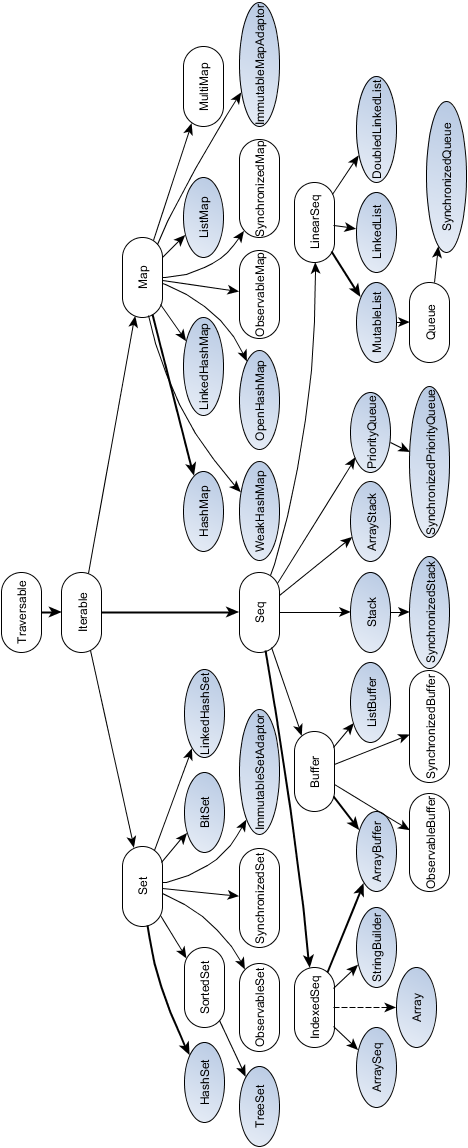
\includegraphics[scale=.60]{scala-collection-mutable.png}
    \captionof{figure}{scala.collection.mutable}
    \label{fig:scala-collection-mutable}
\end{center}


\section{Trait Traversable}


\section{Trait Iterable}


\rule{0.3\linewidth}{0.25pt}
\scriptsize

Copyright \copyright\ 2014 soulmachine

\href{http://www.soulmachine.me}{http://www.soulmachine.me}


\end{multicols}
\end{document}
